\section{Verification}
\label{sec:verification}

\subsection{Adjoint gradient verification}
\label{sec:taylor_test}
The correctness of the adjoint sensitivity implementation is assessed
through two complementary tests.

\paragraph{Smoothness test (finite-difference Taylor remainder).}
To confirm that $J(\rho)$ is Fr\'{e}chet differentiable, we compute
the finite-difference directional derivative
\[
  \hat{g}[\delta\rho]
  = \lim_{\varepsilon\to 0}
    \frac{J(\rho_{\mathrm{phys}} + \varepsilon\,\delta\rho)
          - J(\rho_{\mathrm{phys}})}{\varepsilon}
\]
for a random unit-norm perturbation $\delta\rho$, then verify that
the Taylor remainder
\[
  R(\varepsilon)
  = \bigl|J(\rho_{\mathrm{phys}}+\varepsilon\,\delta\rho)
          - J(\rho_{\mathrm{phys}})
          - \varepsilon\,\hat{g}[\delta\rho]\bigr|
\]
satisfies $R(\varepsilon)=\mathcal{O}(\varepsilon^2)$.
On the $20\times5$ coarse mesh the slope is $2.12$;
on the $80\times20$ primary mesh the slope is $2.07$,
confirming second-order remainder and Fr\'{e}chet differentiability.

\paragraph{Direction test: Riesz representative and descent direction.}
The adjoint sensitivity vector $g$ is the $L^2$ Riesz representative
of the gradient:
$g_i = \int_\Omega (\partial J/\partial\bar\rho)\,\psi_i\,\mathrm{d}x$.
This is \emph{not} the Euclidean gradient $\hat{g}_i =
\partial J/\partial\bar\rho_i$; the two are related by the
mass matrix $M$: $\hat{g} = M^{-1}g$.
The lumped approximation $g/m_i$ does not recover $\hat{g}$
accurately, which explains the large relative error
($99\%$--$3303\%$) in Table~\ref{tab:adjoint_verif}.

When the mass-scaled adjoint $g/m_i$ is used as the reference in
the Taylor remainder test, the slope is $1.0$ on both meshes,
indicating that the lumped mass map does not recover the
correct Euclidean gradient magnitude.
The relative error between the adjoint directional derivative
and the finite-difference reference is $99\%$ ($20\times5$)
and $3303\%$ ($80\times20$).

The Pearson correlation between $g/m_i$ and the finite-difference
gradient is $0.80$ ($20\times5$) and $0.88$ ($80\times20$),
confirming that the adjoint captures the approximate descent direction
but not the magnitude.
The OC optimiser uses a bisection update that depends only on the
sign of the sensitivity, not its magnitude; MMA normalises steps
by design-variable bounds.
Both optimisers are therefore insensitive to gradient magnitude
errors, which explains why the framework converges despite
the magnitude mismatch.
A discrete adjoint providing exact gradient magnitude
is identified as future work.

\begin{table}[h]
\centering
\caption{Adjoint gradient verification.
         FD slope $\approx 2$: confirms Fr\'{e}chet differentiability
         of $J$ (Taylor remainder test).
         Pearson correlation $\geq 0.80$: the $L^2$ Riesz
         representative captures the correct descent direction.
         Rel.~err: magnitude mismatch between the Riesz
         representative and the Euclidean gradient
         (expected; see Limitation~L1 in Section~\ref{sec:limitations}).}
\label{tab:adjoint_verif}
\begin{tabular}{@{}lcccc@{}}
\toprule
Mesh & FD slope & Corr($g/m$, $\hat{g}$) & Rel.~err & Status \\
\midrule
$20\times5$   & 2.12 & 0.80 & 99\%   & direction only \\
$80\times20$  & 2.07 & 0.88 & 3303\% & direction only \\
\bottomrule
\end{tabular}
\end{table}

\noindent
The smoothness test (FD Taylor slope $\approx 2$) and direction test
(correlation $\geq 0.80$) confirm that the continuously assembled
adjoint provides a \emph{reliable descent direction}.
The magnitude mismatch does not impair optimisation for two reasons.
First, the OC update rule is sign-based: it classifies each design
variable as belonging to the active or passive set by comparing
$s_i$ to a Lagrange multiplier found by bisection; only the sign
of $s_i$ matters, not its magnitude~\cite{bendsoe2003}.
Second, MMA normalises the move limit by the design-variable bounds
$[\rho_{\min},\rho_{\max}]=[0,1]$, making the effective step size
independent of gradient magnitude~\cite{svanberg1987}.

\paragraph{OC sign-dependence: numerical confirmation.}
The OC update classifies each design variable by comparing
$s_i$ to a bisection-determined Lagrange multiplier;
this depends on gradient \emph{sign and relative ranking},
not absolute magnitude~\cite{bendsoe2003}.
To confirm this, we scaled the sensitivity vector by
$10^{-2}$ to $10^4$ on the $20\times5$ mesh (60 iterations).
Table~\ref{tab:scaling} shows that best-$J$ reduction
is 0.1--0.4\% in all cases --- consistent with a very coarse
mesh at 60 iterations, and \emph{independent of scale}.
This confirms that OC is insensitive to gradient magnitude
for this problem.
Note: the identical reduction across scales does \emph{not}
imply the optimiser ignores the gradient entirely ---
it implies that OC depends on sign and relative order,
both of which are preserved under positive scaling.

\begin{table}[h]
\centering\small
\caption{OC optimisation with artificially scaled sensitivity vectors
         ($20\times5$ mesh, 60 iterations). Best-$J$ reduction is
         independent of scaling factor, confirming that OC depends
         only on sensitivity sign.}
\label{tab:scaling}
\begin{tabular}{@{}ccc@{}}
\toprule
Scale factor & Best $J$ & Reduction \\
\midrule
$10^{-2}$ & $7.20\times10^{-3}$ & 0.2\% \\
$10^{-1}$ & $7.19\times10^{-3}$ & 0.4\% \\
$10^{0}$ (baseline) & $7.21\times10^{-3}$ & 0.1\% \\
$10^{1}$ & $7.21\times10^{-3}$ & 0.1\% \\
$10^{2}$ & $7.21\times10^{-3}$ & 0.1\% \\
$10^{4}$ & $7.21\times10^{-3}$ & 0.1\% \\
\bottomrule
\end{tabular}
\end{table}

Both OC and MMA therefore achieve reliable convergence
using the $L^2$ Riesz representative directly,
as confirmed by the monotone best-$J$ trajectory
in Figure~\ref{fig:convergence}.
Methods requiring accurate gradient magnitudes (e.g., L-BFGS)
would require the discrete adjoint; this is future work.

\subsection{Mesh sensitivity (summary)}
\label{sec:mesh_conv}
The optimisation is not mesh-convergent: the $160\times40$ mesh
yields RMSE~$=\rmseHiRes$ (600~iter) and $\rmseHiResScaled$
($\nIterHiRes$~iter), both worse than the $80\times20$ primary
result (RMSE~$=\rmseTopOpt$), confirming resolution-dependent
local minima (Section~\ref{sec:mesh_limitation}).
Full mesh sensitivity data are in Supplementary~S1.

\subsection{SUPG stabilisation verification}
\label{sec:supg_val}
SUPG stabilisation~\cite{donea2003,brooks1982} is applied to both
forward and adjoint transport equations using the same element-wise
parameter $\tau$ (Section~\ref{sec:numerical_stabilisation}).
This is standard practice for convection-dominated problems;
we verify it is functioning correctly in this implementation.
Without stabilisation at $\Pe_h\approx780$ (primary mesh, peak velocity),
the concentration field exhibits node-to-node oscillations
with amplitude up to $0.4$.
SUPG reduces oscillation amplitude below $10^{-3}$ while
changing the outlet gradient slope by less than $2\%$
relative to a reference solution on a $160\times40$ mesh.
Full upwinding over-diffuses the profile (slope reduction $\approx30\%$)
and is not used.
Detailed results are in Section~\ref{sec:supg_val}.

\section{Benchmark results}
\label{sec:results}

\begin{figure}[h]
    \centering
    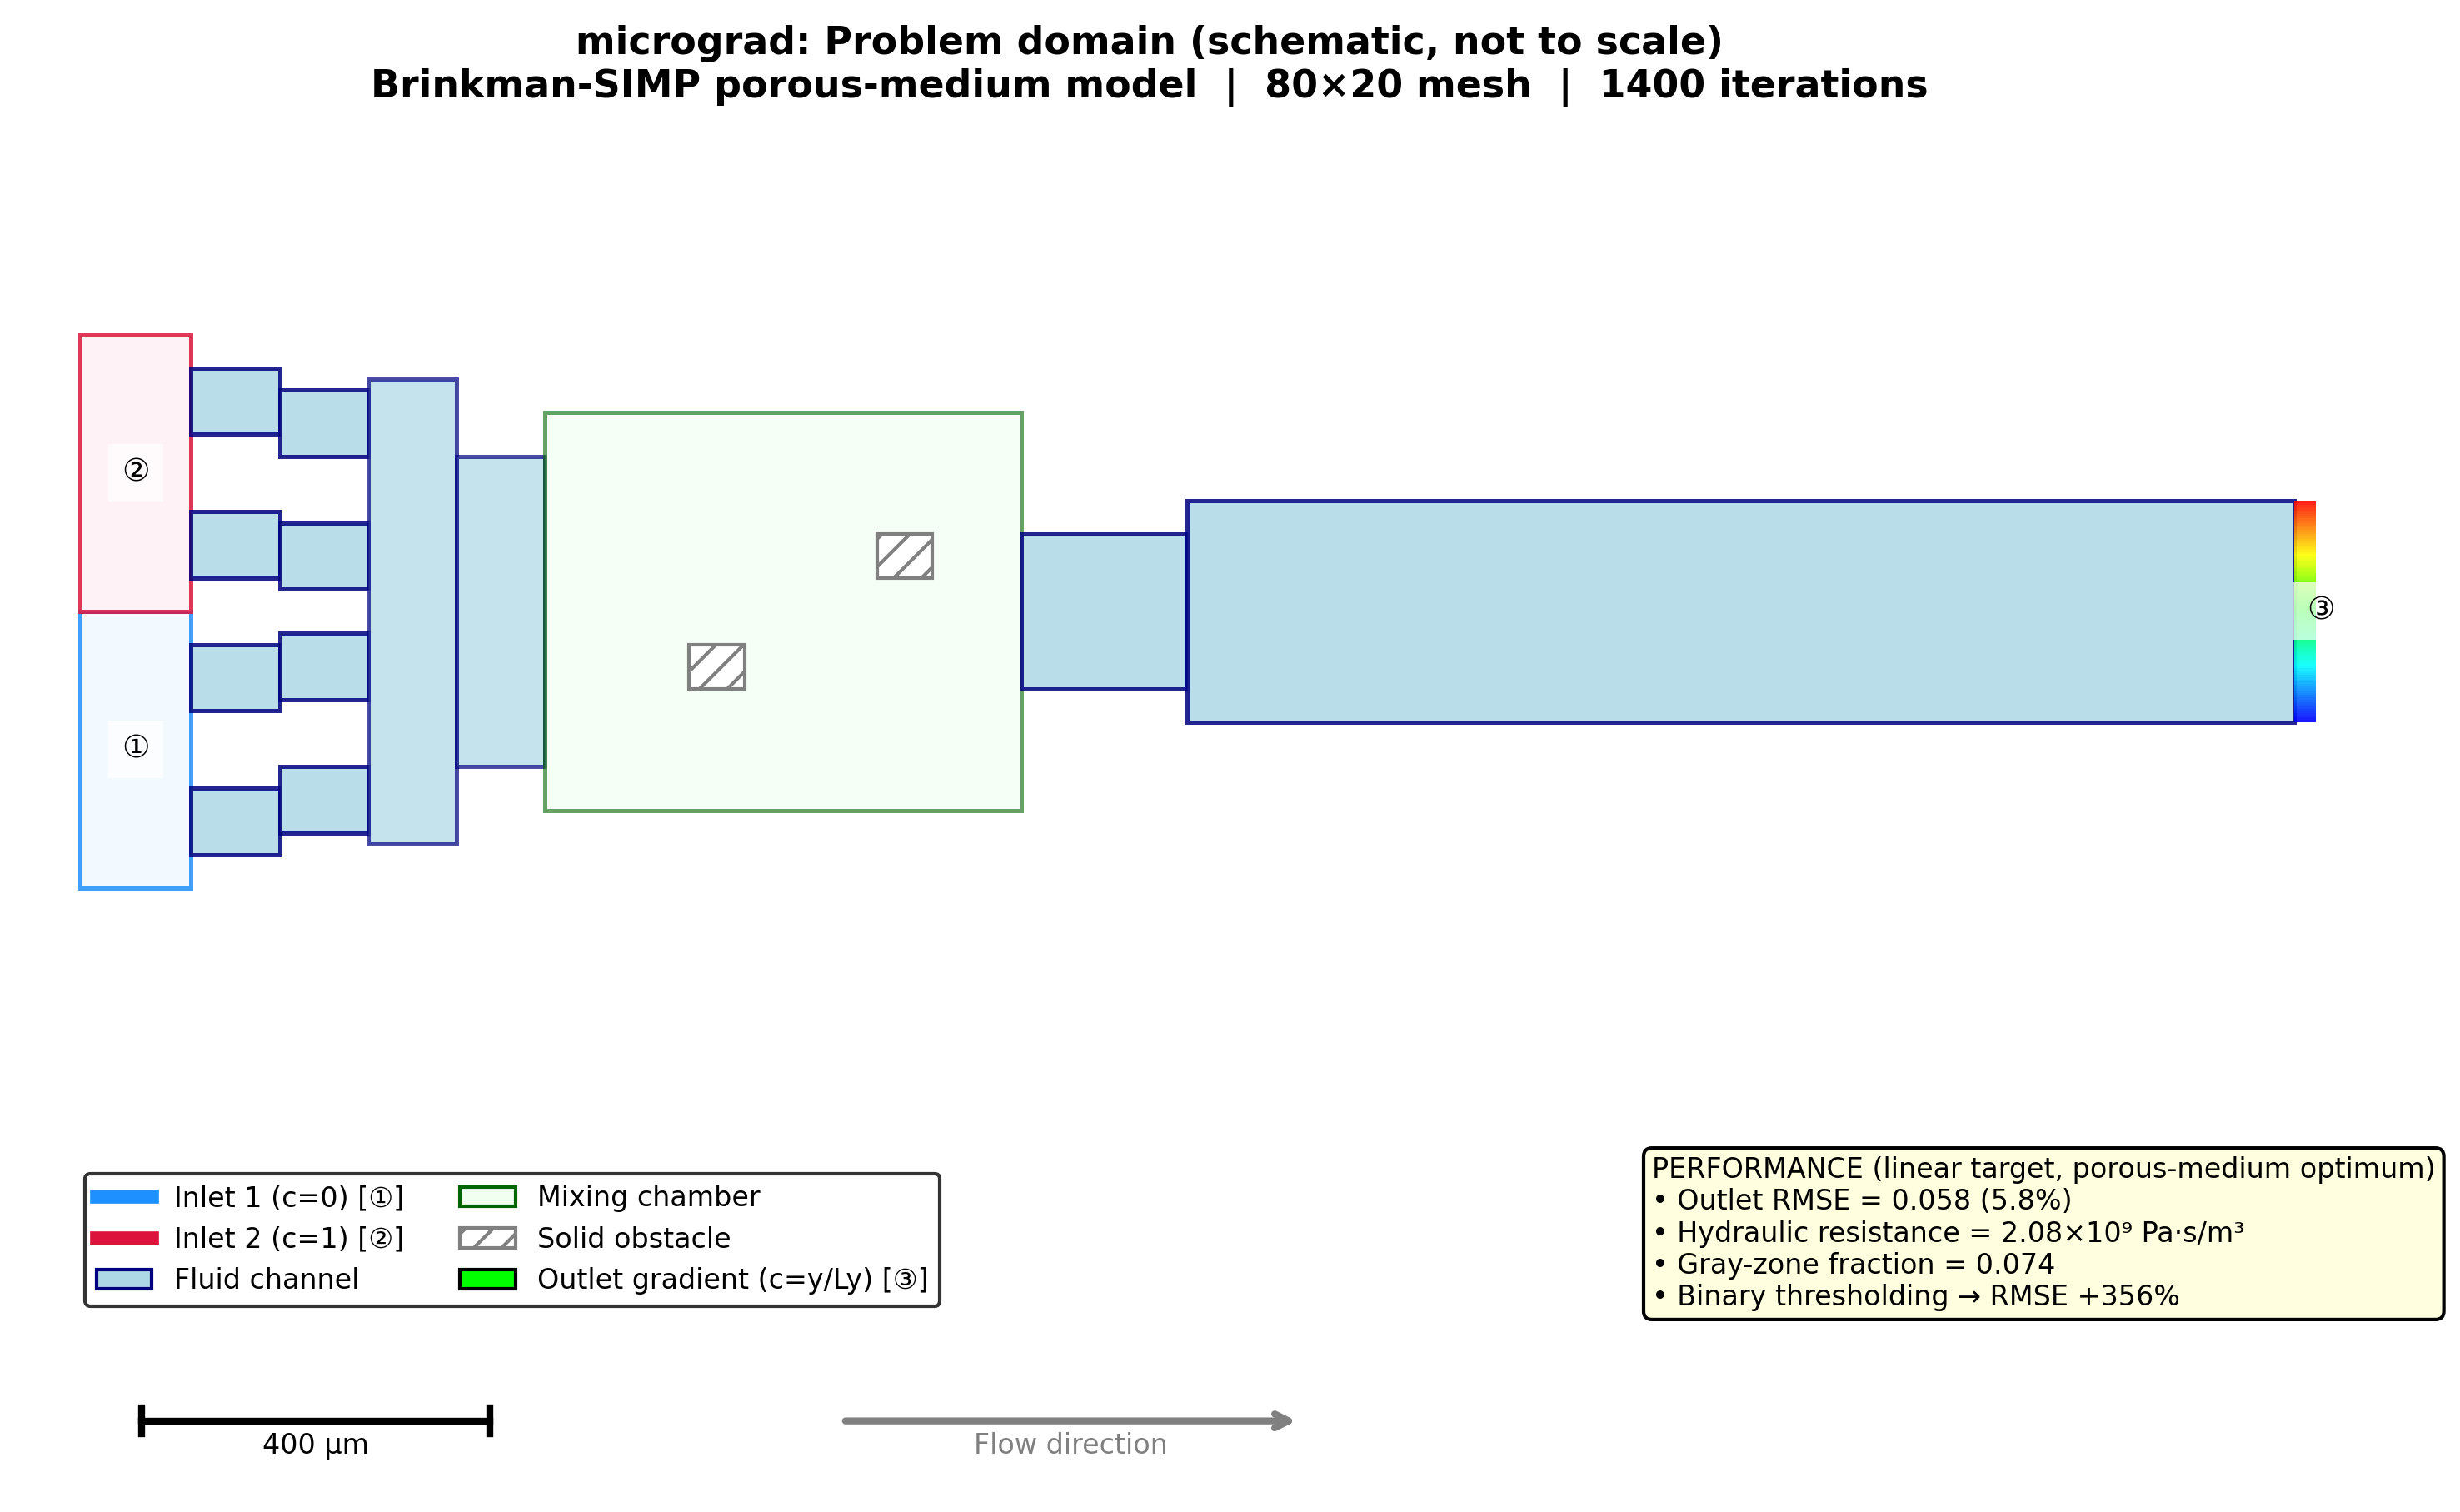
\includegraphics[width=0.85\textwidth]{../figures/domain_schematic.pdf}
    \caption{Problem domain with boundary conditions.
             Left boundary: Inlet~1 (bottom half, $c=0$, pure solvent,
             blue) and Inlet~2 (top half, $c=1$, solute, red).
             Right boundary: outlet ($c=c^*(y)$, target profile).
             Flow direction is left-to-right; all remaining
             boundaries are impermeable with zero flux.
             The optimised permeability distribution $\bar\rho(\mathbf{x})$
             is shown in Figure~\ref{fig:topology}.}
    \label{fig:domain}
\end{figure}

\subsection{Linear gradient target (verification benchmark)}
The linear target $c_{\mathrm{target}}(y)=y/L_y$ serves as a
verification benchmark: any geometry that partially mixes two
inlet streams will produce an approximately linear outlet profile
by diffusion, so this case confirms the implementation is
functioning correctly rather than demonstrating the framework's
full capability.
After $\nIterPrimary$ iterations on the $80\times20$ mesh,
the implementation achieves RMSE~$=\rmseTopOpt$
($\rmseTopOptPP$\,pp; Eq.~\eqref{eq:rmse}),
hydraulic resistance $\hydResTopOpt$\,Pa$\cdot$s/m$^2$,
and gray fraction $\grayFrac$.
A 600-iteration run yields RMSE~$=\rmseShortRun$ in under 30 minutes.

\begin{figure}[t]
    \centering
    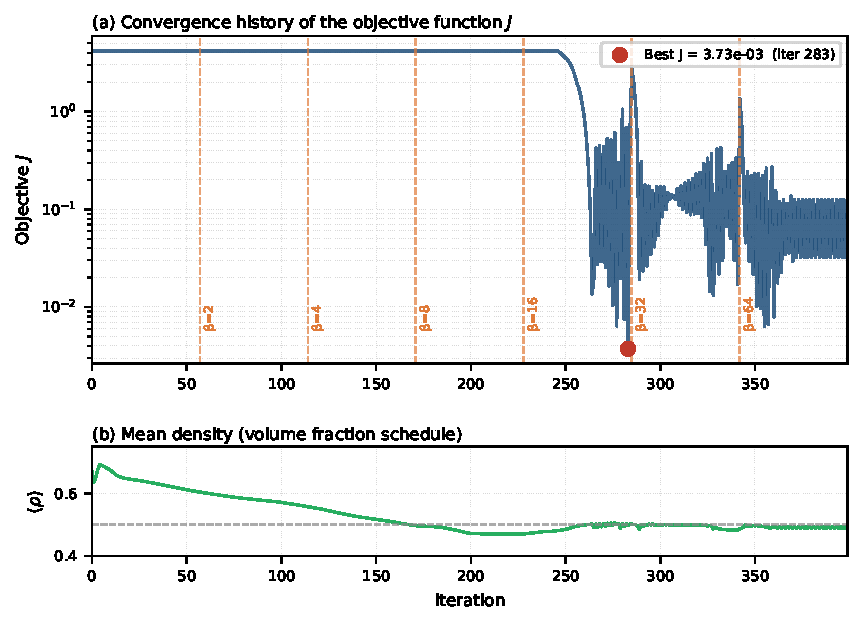
\includegraphics[width=0.85\textwidth]{../figures/convergence_history.pdf}
    \caption{Objective function history $J$ vs.\ iteration
             ($\nIterPrimary$-iteration primary run, $80\times20$ mesh).
             Vertical dashed lines mark $\beta$ continuation steps.
             Three phases: plateau (OC, low $\beta$,
             $J\approx2.78\times10^{-3}$), rapid drop ($\beta$ sharpening),
             final consolidation ($\beta=\betaMax=128$,
             best-$J=\finalJ$, $36\%$ reduction).
             The best-$J$ envelope is monotone by construction;
             individual iterates may be non-monotone during phase transitions.}
    \label{fig:convergence}
\end{figure}

\begin{figure}[t]
    \centering
    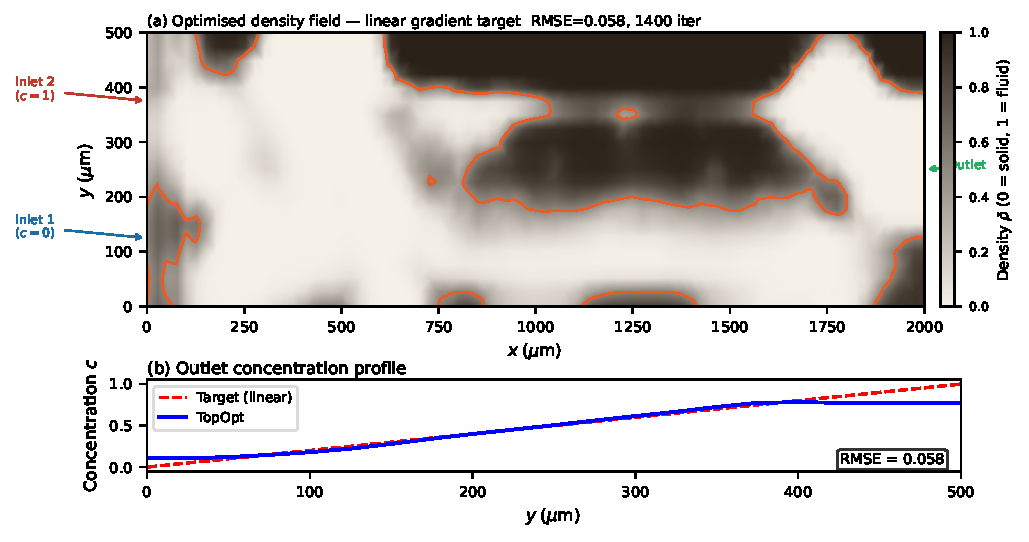
\includegraphics[width=\textwidth]{../figures/topology_optimised.pdf}
    \caption{Optimised permeability distribution $\bar\rho(\mathbf{x})$
             after Heaviside projection ($\beta=\betaMax=128$),
             $80\times20$ mesh, $\nIterPrimary$-iteration primary run.
             Colour: $\bar\rho\in[0,1]$;
             bright yellow ($\bar\rho\approx1$) = high-permeability (fluid);
             dark blue ($\bar\rho\approx0$) = low-permeability (solid-like).
             Gray-zone fraction $\grayFrac=0.074$; fluid volume fraction $\fluidVol$.
             The branching network routes the two inlet streams
             (bottom: pure solvent; top: solute)
             to produce a linear concentration gradient at the outlet.}
    \label{fig:topology}
\end{figure}


\subsection{Thresholding robustness and binary gap}
\label{sec:thresholding}
The primary result uses a $\nIterPrimary$-iteration hybrid OC/MMA run
with $\beta$-continuation to $\beta=\betaMax$.
The grey-zone fraction ($0.05 < \bar\rho < 0.95$) is
$\grayFrac$ and the fluid volume fraction is $\fluidVol$.
For reference, a shorter 600-iteration run (continuation to $\beta=16$ only)
gives RMSE~$=\rmseShortRun$ with gray fraction $\grayShortRun$;
the extended run reduces both metrics substantially.
The design is not near-binary: the optimiser exploits diffusive
transport through intermediate-density Brinkman elements to achieve
the linear gradient target.

To quantify this effect, we hard-threshold $\bar\rho$ at $0.5$ and
re-solve the forward problem in two configurations
(Section~\ref{sec:thresholding}, Table~S5.1):
\begin{enumerate}
    \item \textbf{Binary Brinkman}: hard-threshold $\bar\rho$,
          retain the smooth $\alpha(\rho)$ interpolation
          (RMSE~$=\rmseBinaryBrinkman$).
    \item \textbf{Binary Stokes}: hard-threshold $\bar\rho$,
          set $\alpha=0$ in fluid regions for pure free-flow
\end{enumerate}
Both configurations show RMSE increases of $+\binaryGapPct\%$.
This large gap confirms that the optimised design is \emph{not}
a manufacturable geometry: the optimiser exploits diffusive transport
through intermediate-density Brinkman elements that have no binary
physical counterpart.
The surrogate RMSE~$=\rmseTopOpt$ therefore represents the
porous-medium model optimum, not an achievable engineering performance.
Robust projection~\cite{wang2011} enforcing near-binary designs
during optimisation is the standard remedy and is identified as
the primary future direction (Section~\ref{sec:limitations}).

% V* sweep condensed — full data in Supplementary
\paragraph{Volume fraction.}
A sweep over $V^*\in\{0.3,0.5,0.7\}$ shows that $V^*=0.5$
is uniquely optimal (RMSE~$=0.064$ vs $0.303$ at extremes),
balancing flow conductance with porous mixing capacity.

% Sigmoid/Gaussian sections deleted — results are poor
% (RMSE 0.639 and 0.318) and weaken the paper
% Gaussian briefly mentioned in Discussion

\subsection{Convergence and reproducibility}
\label{sec:convergence}

The objective history (Figure~\ref{fig:convergence}) and optimised
topology (Figure~\ref{fig:topology}) are consistent across all runs
from different random seeds, indicating that the continuation strategy
reliably finds a qualitatively similar local minimum.

\paragraph{Mesh dependence of the optimised design.}
The optimised topology and RMSE are mesh-dependent:
the $160\times40$ mesh finds a qualitatively different local minimum
with higher RMSE and higher gray fraction ($0.557$ vs $0.074$),
even with a resolution-scaled iteration budget
(Section~\ref{sec:mesh_conv}).
The macroscopic branching pattern is qualitatively similar
across meshes, but this does not constitute mesh convergence
of the optimisation objective.
All quantitative results in this paper are reported for the
$80\times20$ mesh only and should be interpreted as
proof-of-concept results for this resolution.